\documentclass[11pt, a4paper]{article}
\pagestyle{empty}
\usepackage{amsmath, amssymb, amsfonts}
\usepackage{setspace}
\usepackage{enumerate}
\usepackage{float}
\usepackage[top=1in, bottom=1in, left=0.5in, right=0.5in, paperwidth=8.5in, paperheight=11in]{geometry}
\usepackage{hyperref}
\usepackage{fullpage}
\usepackage{tikz, pgfplots}
\usepackage{graphicx}
\setstretch{1.2} 
\parindent 0pt

\title{My \LaTeX\ Document}
\author{Chris}
\date{\today}


\def\eq1{y=\dfrac{x}{3x^2+x+1}}
\newcommand{\set}[1]{\setlength\itemsep{#1em}}


\begin{document}
\tableofcontents
\maketitle

Hello! This is my first \LaTeX\ document. 

\ref{fig:example}

% Splited Math Mode with $$ equation $$
$$(x+1)$$\\
\begin{center}
    and
\end{center}
$$(x+3)$$ 

% Inline Math Mode
The equation ${A(x) = x^2 + 4x + 3}$ gives the area of the rectangle. 

Superscripts 
$$2x^{3x + 4}$$
$$2x^{3x^{4+5}}$$

Subscripts
$$x_1$$
$$x_{1_{2_3}}$$
$$a_0, a_1, a_2,\ldots, a_{100}$$

Greek Letters
$$\pi$$
$$\Pi$$
$$\alpha$$
$$A = \pi r^2$$

Trig functions
$$y = \sin x$$
$$y = \cos x$$
$$y = \csc \theta$$
$$y = \sin^{-1} x$$
$$y = \arcsin x$$

Log functions
$$y = \log x$$
$$y = \log_5 x$$
$$y = \ln x$$

Roots
$$\sqrt{4}$$
$$\sqrt[4]{2}$$
$$\sqrt{x^2 + y^4}$$
$$\sqrt{1 + \sqrt{x}}$$

Fractions
% line spacing about this line
$$\frac{2}{2}$$
About $\frac{2}{3}$.
About $\displaystyle \frac{2}{3}$.
About $\dfrac{2}{3}$.

$$\frac{\sqrt{x + 1}}{\sqrt{x + 2}}$$

The distributive property states that $a(b + c) = ab + ac$, for all $a, b, c \in \mathbb{R}$.
The equivalence class of $a$ is $[a]$. 

The set $A$ is defined to be $\{1, 2, 3\}$.

$$\$11.5$$

$$2\left(\frac{1}{x^2-1}\right)$$
$$2\left[\frac{1}{x^2-1}\right]$$
$$2\left\{\frac{1}{x^2-1}\right\}$$
$$2\left\langle\frac{1}{x^2-1}\right\rangle$$
$$2\left|\frac{1}{x^2-1}\right|$$
$$\left.\frac{dy}{dx}\right|_{x=1}$$
$$\left(\frac{1}{1+\left(\frac{1}{1+x}\right)}\right)$$

Table: \par\vspace{6pt}

\begin{tabular}{|c||c|c|r|r|l|}
\hline
$x$ & 1 & 2 & 3 & 4 & 5 \\ \hline
$f(x)$ & 11 & 12 & 13 & 14 & 15 \\ \hline
\end{tabular}

\vspace{1cm}

%% table template
\begin{table}[H]
\centering
\def\arraystretch{1.5}
\begin{tabular}{|c||c|c|r|r|l|}
\hline
$x$ & 1 & 2 & 3 & 4 & 5 \\ \hline
$f(x)$ & $\frac{1}{2}$ & 12 & 13 & 14 & 15 \\ \hline
\end{tabular}
\caption{These values represents the function $f(x)$.}
\end{table}

\vspace{1cm}

\begin{table}[H]
\centering
\def\arraystretch{1.5}
\begin{tabular}{|c|c|}
\hline
$f(x)$ & $f'(x)$ \\ \hline
$x>0$ & The function $f(x)$ is increasing. \\ \hline
\end{tabular}
\caption{The relationship between $f(x)$ and $f'(x)$.}
\end{table}

\vspace{1cm}

\begin{table}[H]
\centering
\def\arraystretch{1.5}
\begin{tabular}{|c|p{2in}|}
\hline
$f(x)$ & $f'(x)$ \\ \hline
$x>0$ & The function $f(x)$ is increasing.  \\ \hline
\end{tabular}
\caption{The relationship between $f(x)$ and $f'(x)$.}
\end{table}

Arrays:
\begin{align}
5x^2-9&=x+3 \\
5x^2-x-12&=0
\end{align}

\begin{align*}
5x^2-9&=x+3 \\
5x^2-x-12&=0
\end{align*}

\begin{enumerate}
    \item pencil
    \item calculator
    \item ruler
    \item notebook
        \begin{itemize}
            \item notes
            \item homework
                \begin{enumerate}
                    \item tests
                    \item quizzes
                \end{enumerate}
        \end{itemize} 
    \item paper
\end{enumerate}

\begin{itemize}
    \item pencil
    \item calculator
    \item ruler
    \item notebook
\end{itemize}

\begin{enumerate}[A.]
    \item a
    \item b
    \item c
\end{enumerate}

\begin{enumerate}[i.]
\set{10}
    \item a
    \item b
    \item c
\end{enumerate}

\pagebreak

\begin{enumerate}\setcounter{enumi}{5}
    \item a
    \item b
    \item c
\end{enumerate}

\begin{itemize}
    \item[] pencil
    \item[] calculator
    \item[] ruler
    \item[] notebook
\end{itemize}

\pagebreak

This will produce \textit{italicized} text. 

This will produce \textbf{bold face} text.
This will produce \textsc{small caps} text. 
This will product \texttt{typewriter font} text.

Please visit Michelle Krummel's website at \href{http://michellekrummel.com}{My Website}.

Please excuse my dear aunt Sally. 

Please excuse my \begin{Large}dear aunt Sally\end{Large}.

Please excuse my \begin{large}dear aunt Sally\end{large}. 

Please excuse my \begin{huge}dear aunt Sally\end{huge}. 

Please excuse my \begin{Huge}dear aunt Sally\end{Huge}. 

\begin{Huge}Please excuse \begin{normalsize}my dear aunt Sally\end{normalsize}\end{Huge}. 

\begin{Huge}Please excuse \begin{small}my dear aunt Sally\end{small}\end{Huge}. 

\begin{Huge}Please excuse \begin{scriptsize}my dear aunt Sally\end{scriptsize}\end{Huge}. 

\begin{Huge}Please excuse \begin{tiny}my dear aunt Sally\end{tiny}\end{Huge}. 

\begin{center}
Center
\end{center}

\begin{flushleft}
Left
\end{flushleft}

\begin{flushright}
Right
\end{flushright}

\pagebreak

\section{Linear Functions}
    \subsection{Slop-Intercept Form}
        \subsubsection{Example1}
        \subsubsection{Example2}
    \subsection{Standard Form}
    \subsection{Point-Slope Form}
\section{Quadratic Functions}

\begin{enumerate}
    \item $\mathbb{R}$
    \item $\mathbb{Z}$
\end{enumerate}

$\eq1$

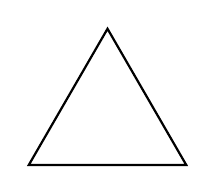
\begin{tikzpicture}
    \draw[thick] (0,0) -- (2,0) -- (1,1.73) -- cycle;
\end{tikzpicture}

% \begin{figure}[H]
%    \centering
%    \includegraphics[width=0.5\linewidth]{Screenshot from %2024-05-22 00-05-18.png}
%    \caption{This is picture example.}
%    \label{fig:example}
% end{figure}

\begin{tikzpicture}
    % 绘制坐标轴
    \draw[->] (-3,0) -- (3,0) node[right] {$x$}; % x 轴
    \draw[->] (0,-3) -- (0,3) node[above] {$y$}; % y 轴

    % 绘制一条从 (-2, -1) 到 (2, 2) 的直线
    \draw[thick, blue] (-2,-1) -- (2,2) node[above] {$(2,2)$};
    
    % 在坐标轴上标记点
    \draw[fill] (-2,-1) circle [radius=2pt] node[below left] {$(-2,-1)$};
    \draw[fill] (2,2) circle [radius=2pt] node[above right] {$(2,2)$};
    
    % 绘制函数 y = x 的图像
    \draw[red, thick, domain=-2.5:2.5] plot (\x, \x) node[right] {$y=x$};
\end{tikzpicture}


\end{document}
